\begin{frame}
\frametitle{Definições}
	
Artigo referenciado:

\medskip

\textbf{O. Sorkine}, \textit{Differential representations for mesh processing}, Computer Graphics Forum, (2006) \cite{sorkine2006}.
	
\end{frame}

\begin{frame}
\frametitle{Coordenadas diferenciais}

Seja uma malha triangular $\mathcal{M} = (V, E, F)$. Cada vértice $\mathbf{v}_i \in V$ possui uma representação cartesiana dada por $\mathbf{v}_i = (x_i,y_i,z_i)$.

\medskip

\destaq{Coordenadas diferenciais} (ou $\mathbf{\delta}$\textit{-coordenadas}) de $\mathbf{v}_i$ são definidas como a diferença entre a coordenada cartesiana e o centro de massa de seus vizinhos imediatos na malha:

\begin{equation}
\mathbf{\delta}_i = (\mathbf{\delta}_i^{(x)}, \mathbf{\delta}_i^{(y)}, \mathbf{\delta}_i^{(z)}) = \mathbf{v}_i - \frac{1}{d_i} \sum_{j \in N(i)} \mathbf{v}_j,
\label{eq_delta}
\end{equation}

\noindent em que $N(i) = \{j|(i,j) \in E$\} e $d_i = |N(i)|$.
	
\end{frame}




\begin{frame}
\frametitle{Coordenadas diferenciais}
\framesubtitle{Transformação para $\delta$-coordenadas}

Seja $A$ a matriz de adjacências da malha:

$$
A_{ij} = \begin{cases}
1&(i, j) \in E\\
0&\text{caso contrário.}
\end{cases}
$$

e $D$ a matriz diagonal tal que

$$D_{ii} = d_{i} = |N(i)| = \text{número de vértices adjacentes a }i$$

A matriz $L$ de transformação de coordenadas cartesianas para as coordenadas diferenciais é:

\begin{equation}
L = I - D^{-1}A.
\end{equation}
	
\end{frame}

\begin{frame}
\frametitle{Coordenadas diferenciais}
\framesubtitle{Transformação para $\delta$-coordenadas}

É mais comum utilizar a versão simétrica de $L$, $L_s$, tal que:

$$L_s = DL = D - A$$

e cada célula pode ser calculada por:

\begin{equation}
(L_s)_{ij} = \begin{cases}
d_i&i=j\\
-1&(i, j) \in E\\
0&\text{caso contrário.}
\end{cases}
\end{equation}

	
\end{frame}

\begin{frame}
\frametitle{Coordenadas diferenciais}
\framesubtitle{Transformação para $\delta$-coordenadas}

Temos:

$$L_s \textbf{x} = \delta^{(x)}$$
$$L_s \textbf{y} = \delta^{(y)}$$
$$L_s \textbf{z} = \delta^{(z)}$$

e $L_s$ é denominado \destaq{Laplaciano topológico} da malha $\mathcal M$.

\end{frame}

\begin{frame}
\frametitle{Coordenadas diferenciais}
\framesubtitle{Discretização de Laplace-Beltrami}

Se considerar $\mathcal{M}$ uma aproximação linear por partes de uma superfície suave,

$$\delta_i = \frac{1}{d_i} \sum_{j \in N(i)}(\mathbf{v_i} - \mathbf{v_j})$$

é uma discretização de

$$\frac{1}{|\gamma|} \int_{v \in \gamma} (v_i - v) dl(v)$$

em que $\gamma$ é uma curva de uma superfície fechada simples em volta de $v_i$ e $|\gamma|$ é o comprimento de $\gamma$.

\end{frame}

\begin{frame}
\frametitle{Coordenadas diferenciais}
\framesubtitle{Discretização de Laplace-Beltrami}

Sabe-se que:

$$\lim\limits_{|\gamma|\rightarrow 0} \frac{1}{|\gamma|} \int_{v \in \gamma} (v_i - v) dl(v) = - H(v_i) n_i$$

em que $H(v_i)$ é a curvatura média de $v_i$ e $n_i$ é a normal à superfície.

\medskip

Intuitivamente, as $\delta$-coordenadas \destaq{encapsulam a forma local da superfície}.

\end{frame}

\begin{frame}
\frametitle{Reconstrução de $v_i$}
\framesubtitle{A partir das $\delta$-coordenadas}

$$L_s \textbf{x} = \delta^{(x)}$$

\begin{itemize}
\item $\delta$-coordenadas são invariantes à translação;
\item $L$ e $L_s$ são singulares;
\item $\textbf{x} = L_s^{-1} \delta^{(x)}$ é \textbf{indefinido}.
\item \textbf{Solução:} adicionar restrições de quem se conhece a localização.

\end{itemize}

\end{frame}


\begin{frame}
\frametitle{Reconstrução de $v_i$}
\framesubtitle{A partir das $\delta$-coordenadas}

$$L_s \textbf{x} = \delta^{(x)}$$

\begin{itemize}
\item $rank(L) = n - k$, em que $k$ é o número de componentes;
\item Fixar vértices $C = \{1, 2, \dots, m\}$, em que sabe-se $\{v_{C_1}, v_{C_2}, \dots, v_{C_m}\}$;
\item Ou seja, adicionar restrições $v_{j} = c_j,\ j \in C$;
\item Tornando o sistema \textit{full-rank}.
\end{itemize}
	
\end{frame}


\begin{frame}
\frametitle{Reconstrução de $v_i$}
\framesubtitle{A partir das $\delta$-coordenadas}

Fixar vértices $C = \{1, \dots, m\}$ em que sabe-se $\{v_{C_1}, v_{C_2}, \dots, v_{C_m}\}$:

\bigskip

$$\left(\frac{L}{I_{m\times m} | 0}\right) \textbf{x} = \begin{pmatrix}
\delta^{(x)} \\
c_{1:m}
\end{pmatrix}$$

\bigskip
\medskip
\smallskip

\end{frame}


\begin{frame}
\frametitle{Reconstrução de $v_i$}
\framesubtitle{A partir das $\delta$-coordenadas}


Inicialmente, tem-se:

\bigskip

\begin{center}
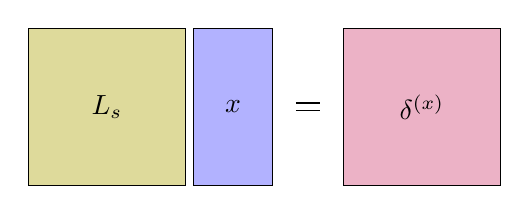
\begin{tikzpicture}
\filldraw[fill=olive!30!white, draw=black] (0,0) rectangle node{$L_s$} (2,2);
\filldraw[fill=blue!30!white, draw=black] (2.1,0) rectangle node{$x$} (3.1,2);
\draw (3.4, 0.95) -- (3.7, 0.95);
\draw (3.4, 1.05) -- (3.7, 1.05);
\filldraw[fill=purple!30!white, draw=black] (4,0) rectangle node{$\delta^{(x)}$} (6,2);
\end{tikzpicture}
\end{center}

\bigskip
\medskip
\smallskip

\end{frame}

\begin{frame}
\frametitle{Reconstrução de $v_i$}
\framesubtitle{A partir das $\delta$-coordenadas}

Fixar vértices $C = \{1, \dots, m\}$ em que sabe-se $\{v_{C_1}, v_{C_2}, \dots, v_{C_m}\}$:

\bigskip

\begin{center}
	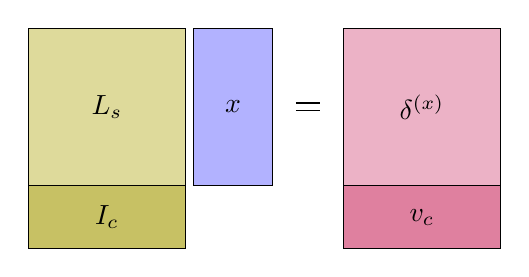
\begin{tikzpicture}
	\filldraw[fill=olive!30!white, draw=black] (0,0) rectangle node{$L_s$} (2,2);
	\filldraw[fill=olive!50!white, draw=black] (0,0) rectangle node{$I_c$} (2,-0.8);
	\filldraw[fill=blue!30!white, draw=black] (2.1,0) rectangle node{$x$} (3.1,2);
	\draw (3.4, 0.95) -- (3.7, 0.95);
	\draw (3.4, 1.05) -- (3.7, 1.05);
	\filldraw[fill=purple!30!white, draw=black] (4,0) rectangle node{$\delta^{(x)}$} (6,2);
	\filldraw[fill=purple!50!white, draw=black] (4,0) rectangle node{$v_c$} (6,-0.8);
	\end{tikzpicture}
\end{center}

\end{frame}

\begin{frame}
\frametitle{Reconstrução de $v_i$}
\framesubtitle{A partir das $\delta$-coordenadas}

Fixar vértices $C = \{1, \dots, m\}$ em que sabe-se $\{v_{C_1}, v_{C_2}, \dots, v_{C_m}\}$:

\bigskip

\begin{center}
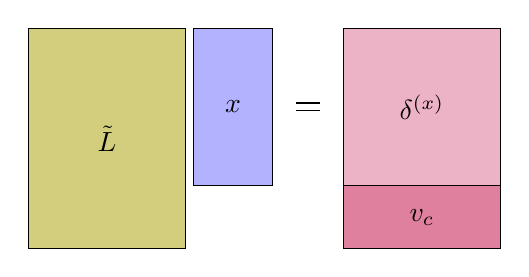
\begin{tikzpicture}
\filldraw[fill=olive!40!white, draw=black] (0,-0.8) rectangle node{$\tilde{L}$} (2,2);
\filldraw[fill=blue!30!white, draw=black] (2.1,0) rectangle node{$x$} (3.1,2);
\draw (3.4, 0.95) -- (3.7, 0.95);
\draw (3.4, 1.05) -- (3.7, 1.05);
\filldraw[fill=purple!30!white, draw=black] (4,0) rectangle node{$\delta^{(x)}$} (6,2);
\filldraw[fill=purple!50!white, draw=black] (4,0) rectangle node{$v_c$} (6,-0.8);
\end{tikzpicture}
\end{center}


\end{frame}

\begin{frame}
\frametitle{Reconstrução de $v_i$}
\framesubtitle{A partir das $\delta$-coordenadas}

\begin{figure}
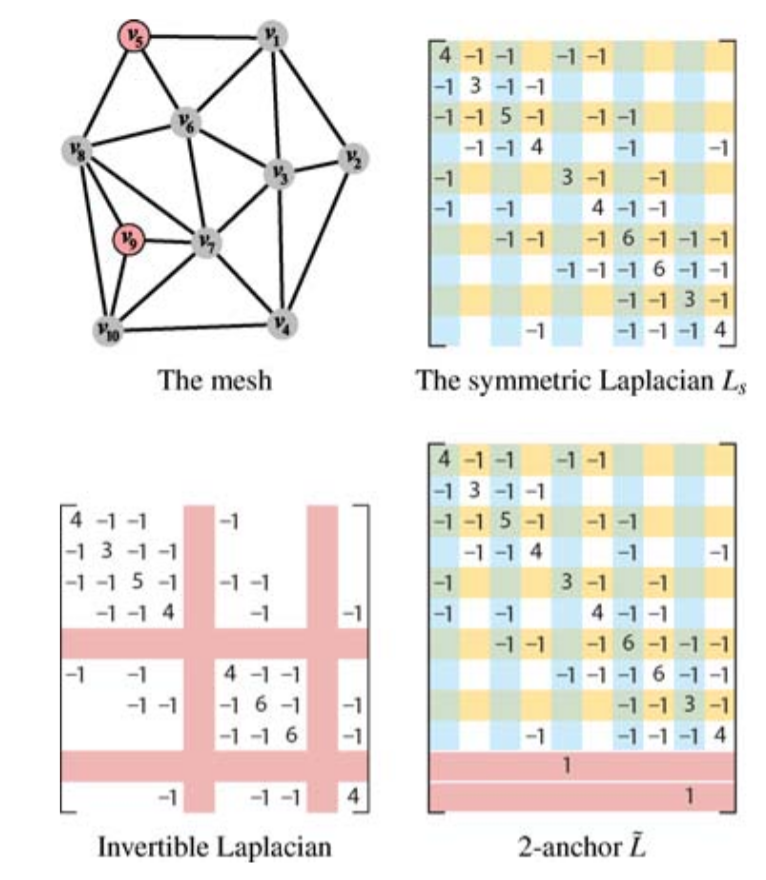
\includegraphics[width=0.5\linewidth]{img/lrestricao.png}
\caption{Exemplo da matriz $\tilde{L}$ \cite{sorkine2006}}
\end{figure}

\end{frame}